% XCircuit output "challenge.tex" for LaTeX input from challenge.ps
\def\putbox#1#2#3#4{\makebox[0in][l]{\makebox[#1][l]{}\raisebox{\baselineskip}[0in][0in]{\raisebox{#2}[0in][0in]{\scalebox{#3}{#4}}}}}
\def\rightbox#1{\makebox[0in][r]{#1}}
\def\centbox#1{\makebox[0in]{#1}}
\def\topbox#1{\raisebox{-0.60\baselineskip}[0in][0in]{#1}}
\def\midbox#1{\raisebox{-0.20\baselineskip}[0in][0in]{#1}}
\begin{center}
   \scalebox{1}{
   \normalsize
   \parbox{4.5in}{
   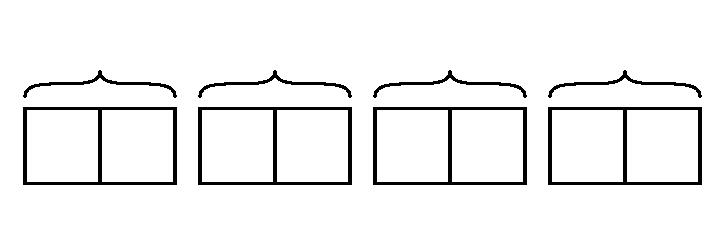
\includegraphics[scale=1]{challenge.ps}\\
   % translate x=624 y=285 scale 0.38
   \putbox{0.31in}{0.12in}{1.20}{\centbox{\midbox{0}}}%
   \putbox{0.81in}{0.12in}{1.20}{\centbox{\midbox{1}}}%
   \putbox{1.47in}{0.12in}{1.20}{\centbox{\midbox{2}}}%
   \putbox{1.97in}{0.12in}{1.20}{\centbox{\midbox{3}}}%
   \putbox{2.64in}{0.12in}{1.20}{\centbox{\midbox{4}}}%
   \putbox{3.14in}{0.12in}{1.20}{\centbox{\midbox{5}}}%
   \putbox{3.81in}{0.12in}{1.20}{\centbox{\midbox{6}}}%
   \putbox{4.31in}{0.12in}{1.20}{\centbox{\midbox{7}}}%
   \putbox{0.56in}{1.29in}{1.20}{\centbox{\midbox{OPCODE}}}%
   \putbox{1.72in}{1.29in}{1.20}{\centbox{\midbox{A}}}%
   \putbox{2.89in}{1.29in}{1.20}{\centbox{\midbox{B}}}%
   \putbox{4.06in}{1.29in}{1.20}{\centbox{\midbox{A ? B}}}%
   } % close 'parbox'
   } % close 'scalebox'
   \vspace{-\baselineskip} % this is not necessary, but looks better
\end{center}
